\documentclass{standalone}
%outline around text
\usepackage[outline]{contour}
\contourlength{1.3pt}

%tikz
\usepackage{tikz}
\usetikzlibrary{knots, cd, calc}

\begin{document}


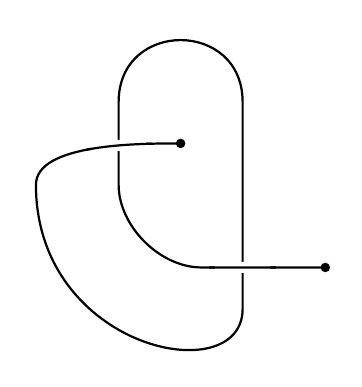
\begin{tikzpicture}[scale = 1.05]
\clip (-1.1, -2.1) rectangle (2.6, 1.9);
\begin{knot}[clip width = 5, consider self intersections = true, ignore endpoint intersections = false, flip crossing = 2
]
\strand[thick] 
	(2.5, -1)  -- 
	(1, -1) .. controls +(-.5, 0) and +(0, -.5) ..
	(0, 0) -- 
	(0, 1) .. controls +(0, 1) and +(0, 1) ..
	(1.5, 1) --
	(1.5, -1.5) .. controls +(0, -1) and +(0, -2) ..
	(-1, 0) .. controls +(0, 0.5) and +(-.5, 0) ..
	(0.75, 0.5);
\end{knot}
\draw[fill = black] (0.75, 0.5) circle (0.05);
\draw[fill = black] (2.5, -1) circle (0.05);
\end{tikzpicture}


\end{document}